\subsubsection{\stid{4.15} ExaHDF5}\label{subsubsect:exahdf5}

\paragraph{Overview} 

Hierarchical Data Format version 5 (HDF5) is the most popular high-level I/O library for scientific applications to write and read data files. The HDF Group released the first version of HDF5 in 1998 and over the past 20 years, it has been used by numerous applications not only in scientific domains but also in finance, space technologies, and many other business and enginering fields. HDF5 is the most used library for performing parallel I/O on existing HPC systems at the DOE supercomputing facilities. NASA gives HDF5 software the highest technology readiness level (TRL 9), which is given to actual systems ``flight proven'' through successful mission operations. 

In this project, we have developed various HDF5 features are in development to address efficiency and other challenges posed by data management and parallel I/O on exascale architectures. The ExaIO-HDF5 team is productizing features and techniques that have been previously prototyped, exploring optimization strategies on upcoming architectures, maintaining and optimizing existing HDF5 features tailored for ECP applications. Along with supporting and optimizing I/O performance of HDF5 applications, new features in this project include transparent data caching in the multi-level storage hierarchy, topology-aware I/O related data movement in exascale systems, full single-writer and multi-reader (SWMR) for workflows, asynchronous I/O, querying data and metada, and sub-filing. 

Many of the funded exascale applications and co-design centers require HDF5 for their I/O, and enhancing the HDF5 software to handle the unique challenges of exascale architectures will play an instrumental role in the success of the ECP. For instance, AMReX, the AMR co-design center is using HDF5 for I/O, and all the ECP applications that are collaborating with AMReX will benefit from improvements to HDF5. The full SWMR feature will support the needs of ExaFEL’s workflow in appending data incrementally. The virtual Object Layer (VOL) and interoperability features with netCDF and ADIOS data open up the rich HDF5 data management interface to a large number of file formats. The project will be releasing these new features in HDF5 for broad deployment on HPC systems. Focusing on the challenges of exascale I/O, technologies will be developed based on the massively parallel storage hierarchies that are being built into pre-exascale systems. The enhanced HDF5 software will achieve efficient parallel I/O on exascale systems in ways that will impact a large number of DOE science as well as industrial applications.

\paragraph{Key  Challenges}
\paragraph{}
There are challenges in developing I/O strategies for using a hierarchy of storage devices and topology of compute nodes efficiently, developing interoperability features with other file formats, and integrating existing prototyped features into production releases. 

\textit{Efficient use of hierarchical storage and topology.} Data generation (e.g., by simulations) and consumption (such as for analysis) in exascale applications may span various storage and memory tiers, including near-memory NVRAM, SSD-based burst buffers, fast disk, campaign storage, and archival storage. Effective support for caching and prefetching data based on the needs of the application is critical for scalable performance. Also, support for higher bandwidth transfers and lower message latency interconnects in supercomputers are becoming more complex, in terms of both topology as well as routing policies. I/O libraries need to fully account for this topology in order to maximize I/O performance, and current I/O mechanisms fail to exploit the system topology efficiently.

%\textit{Interoperability with other file formats.} HDF5 offers a rich data model and powerful features for operating on data, and using these capabilities to access data stored in other data formats would be a valuable productivity boost to application developers and workflows. The team is developing  interoperability features that will enable ECP applications to use HDF5 function calls to read data directly from other file formats. Development includes functionality to read “classic” netCDF (including PnetCDF) and ADIOS/BP files, as these formats are in active use in DOE application communities focused on exascale deliverables. 

\textit{Asynchronous I/O}: Asynchronous I/O allows an application to overlap I/O with other operations. When an application properly combines asynchronous I/O with nonblocking communication to overlap those operations with its calculation, it can fully utilize an entire HPC system, leaving few or no system components idle.  Adding asynchronous I/O to an application's existing ability to perform nonblocking communication is a necessary aspect of maximizing the utilization of valuable exascale computing resources.


\paragraph{Solution Strategy}

\textit{Utilizing complex compute and storage hardware. } Data Elevator is being developed in this project to exploit multi-level storage hierarchies. The Data Elevator library intercepts HDF5 file access calls and redirects them to intermediate faster caching storage layers, which future application reads or writes will then access. When updates or writes to the intermediate data are finished, Data Elevator's server daemon moves the data transparently to its final destination on colder storage layers, such as disk-based parallel file system.  This occurs transparently to the application, without modifying the source code or placing a burden on user to move the data explicitly to and from the intermediate caching storage layer.

In our prior work, improved communication times were achieved for a wide spectrum of data movement patterns such as those seen in multi-physics codes, parallel I/O aggregation, and in situ analysis, and have also improved the time to access parallel file systems. The team is developing these topology-aware optimization strategies as a Virtual File Driver (VFD), which can be plugged in to HDF5. 

\begin{wrapfigure}{r}{0.51\textwidth}
  \begin{center}
    %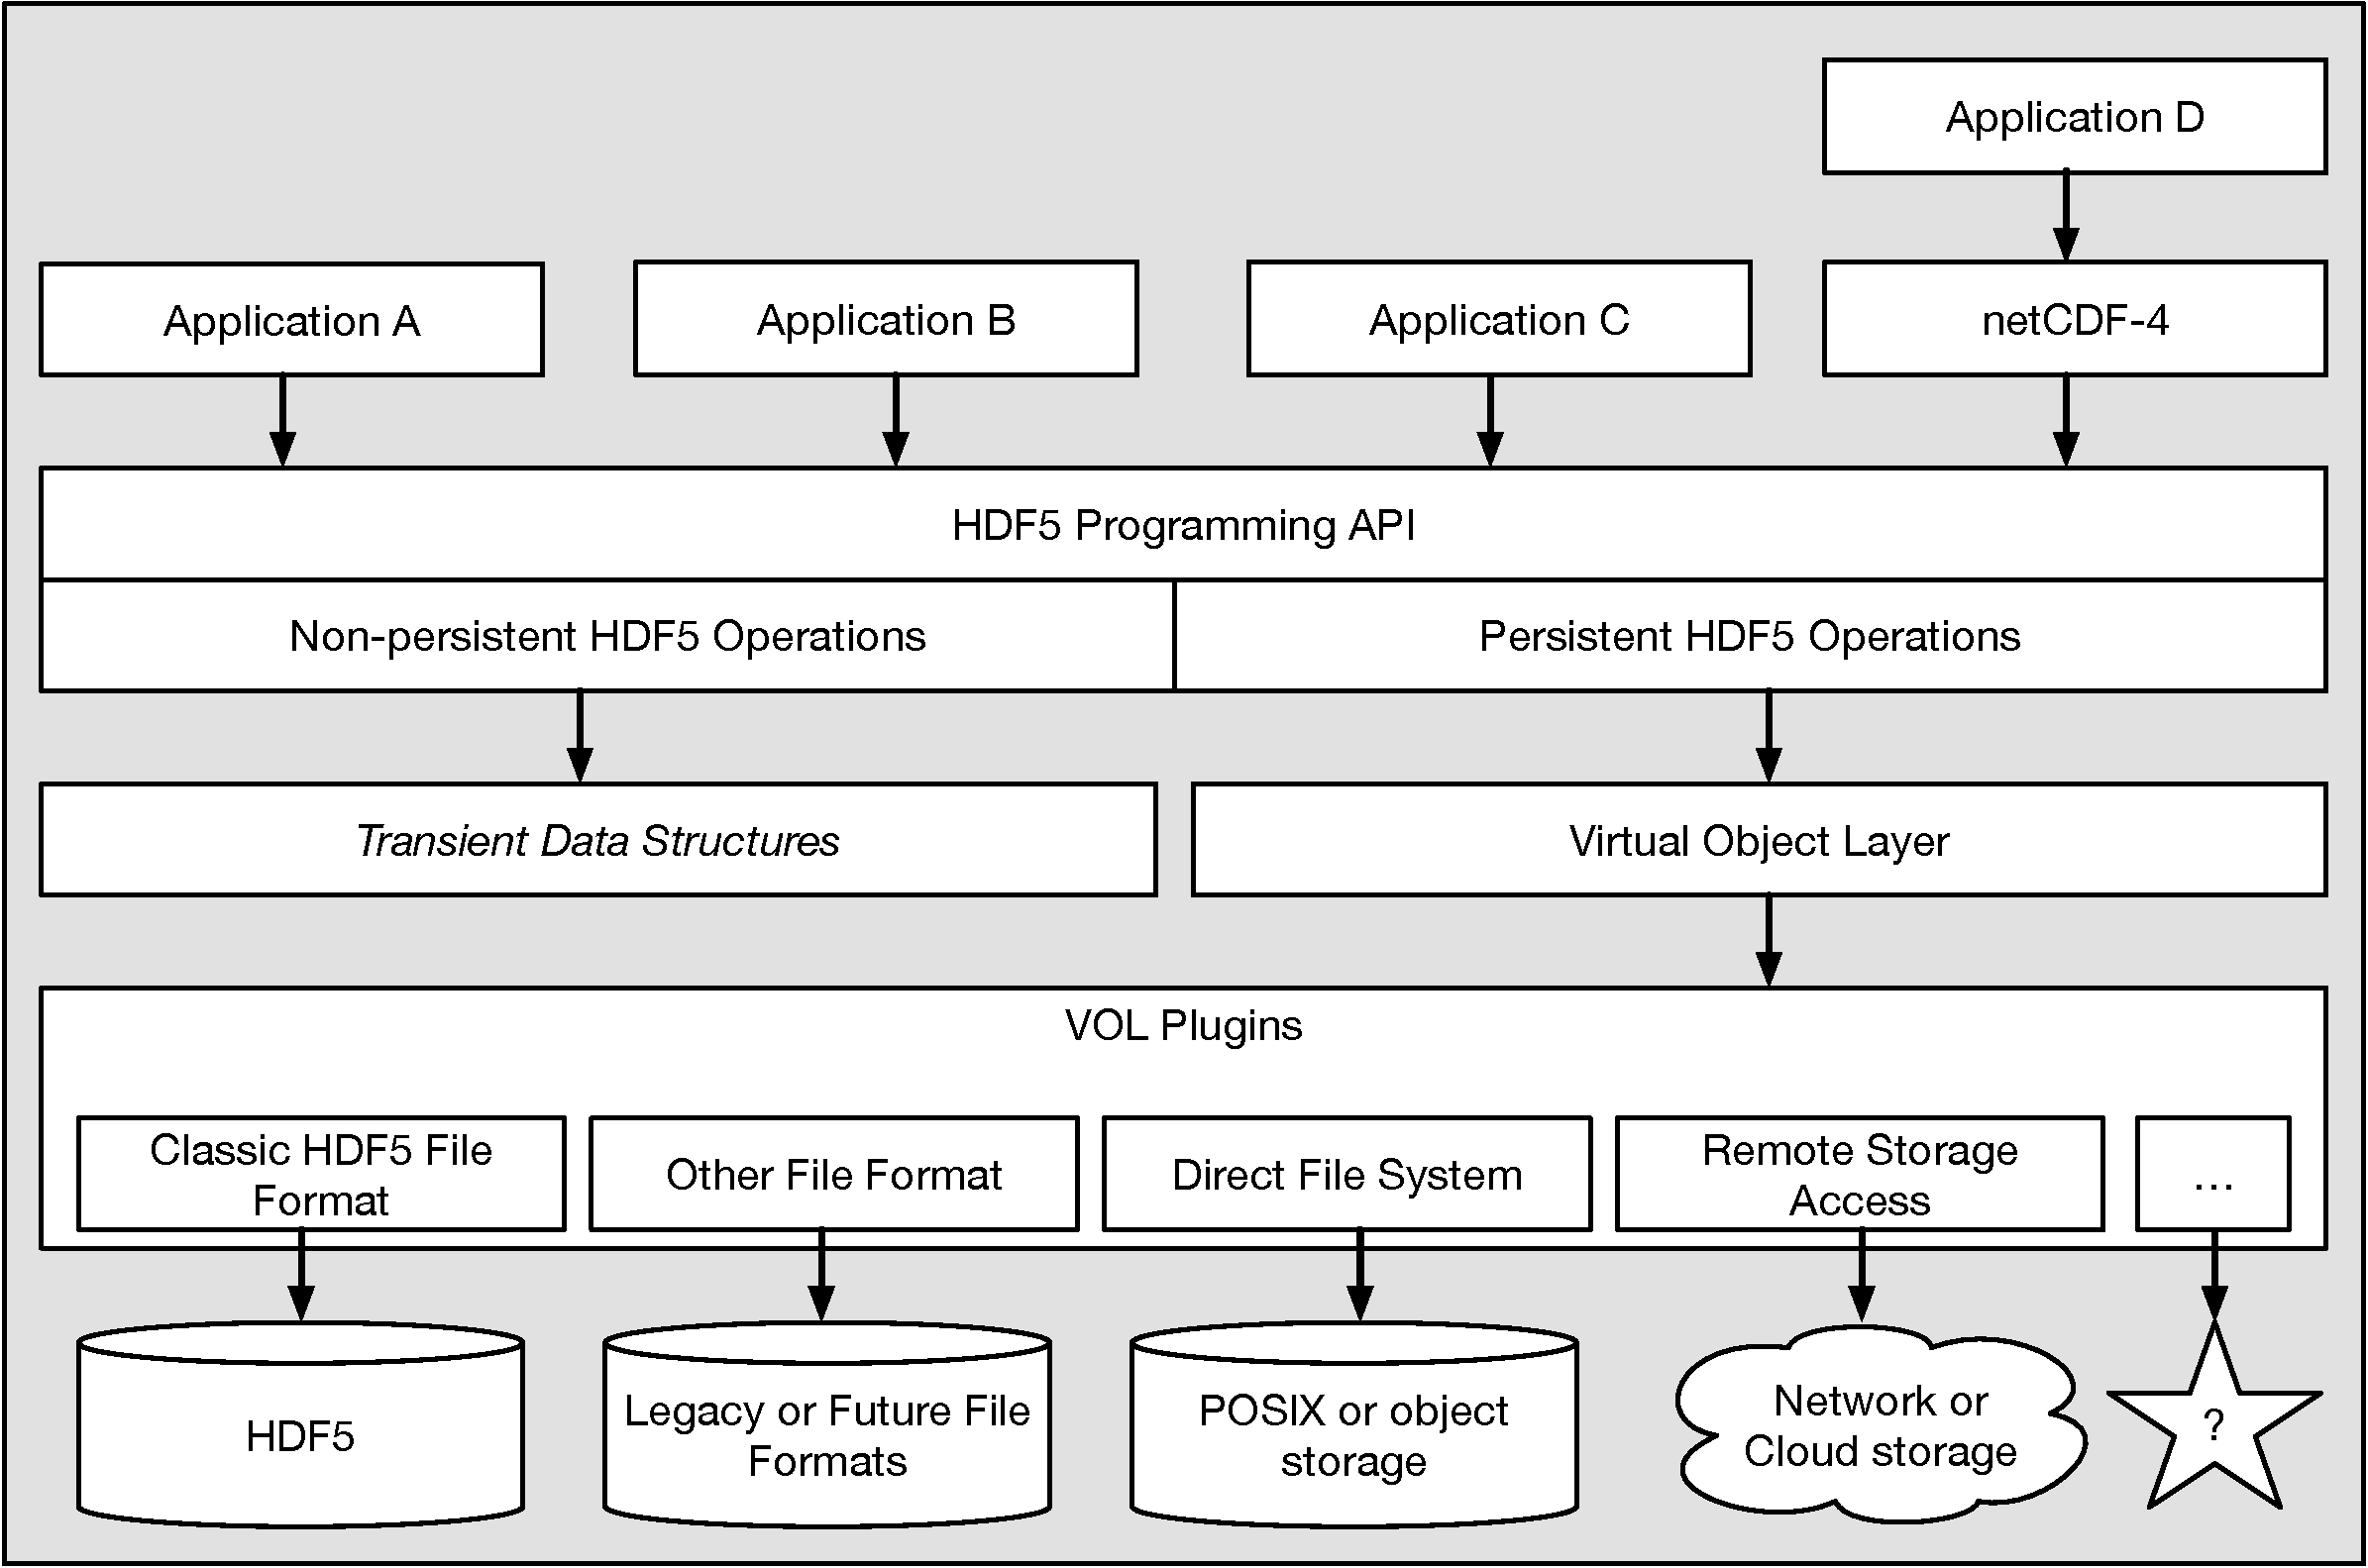
\includegraphics[width=0.48\textwidth]{projects/2.3.4-DataViz/2.3.4.15-HDF5-UnifyCR/VOL-Overview.pdf}
    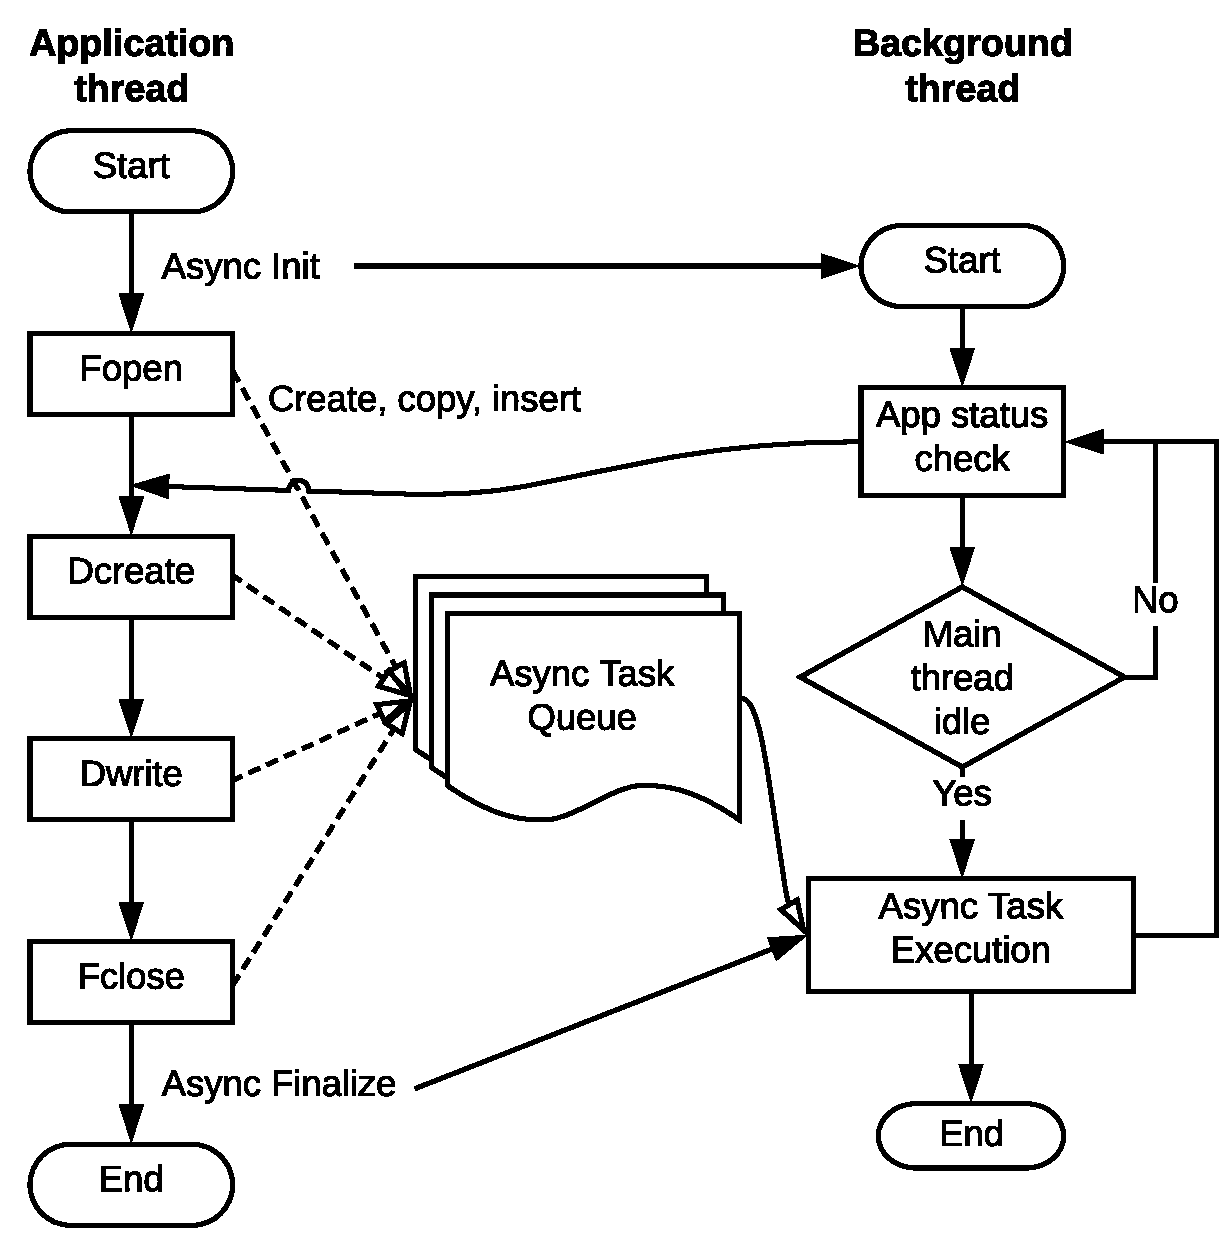
\includegraphics[width=0.48\textwidth]{projects/2.3.4-DataViz/2.3.4.15-HDF5-UnifyCR/async_io_overview.pdf}
  \end{center}
  \caption{An overview of asynchronous I/O as a HDF5 VOL connector}
  \label{fig:asyncio-overview}
\end{wrapfigure}

%\textit{Interoperability with other file formats.} To open the HDF5 API for interfacing with various file formats and to provide the capability of intercepting HDF5 API calls, a ``Virtual Object Layer'' (VOL) feature is being developed. The VOL adds a new abstraction layer internally within the HDF5 library and is implemented just below the public API. The VOL intercepts all HDF5 API calls that access objects in a file and forwards those calls to an “object connector”, which can be pre-linked, or loaded dynamically. A VOL connector can store HDF5 data model objects in a variety of ways. Figure \ref{fig:vol-overview} shows a high-level view of the VOL, where intercepted HDF5 API calls can interface with other file formats and object storage. We will create VOL connectors to access the netCDF and ADIOS/BP file formats, so that applications can use the HDF5 API to operate on data stored in these formats. The interoperability functions in the VOL support the pre-defined datatypes (integers, floating-point values, strings, etc.) in these formats, and will also support compound datatypes, i.e., a user-defined combination of pre-defined datatypes, in netCDF and will use compound datatypes to support ADIOS’ complex datatypes, which represent complex numbers.

\textit{Asynchrnous I/O Virtual Object Layer (VOL) Connector}: Implementation of asynchronous I/O operations can be achieved in different ways. Since the native asynchronous interface offered by most existing operating systems and low-level I/O frameworks (POSIX AIO and MPI-IO) does not include all file operations, we chose to perform I/O operations in a background thread. With recent increase in the number of available CPU threads per processor, it is now possible to use a thread to execute asynchronous operations from the core that the application is running on without significant impact to the application's performance. As shown in Figure \ref{fig:asyncio-overview}, when an application enables asynchronous I/O, a background thread is started. Each I/O operation is intercepted and an asynchronous task is created, storing all the relevant information before inserting it into the asynchronous task queue. The background thread monitors the running state of the application, and only starts executing the accumulated tasks when it detects the application is idle or performing non-I/O operations. When all I/O operations have completed and the application issues the file close call, the asynchronous I/O related resources, as well as the background thread itself, would be freed.

\paragraph{Recent Progress}
\emph{Prototype implementation of Data Elevator read prefetching.} The project team has developed a prototype implementation of read caching and prefetching functionality and tested with various data read kernels from real applications. Using the burst buffers on Cori, the Data Elevator achieves 1.2--3X performance improvement over a highly tuned HDF5 code in reading data. Performance evaluation included representative I/O of convolution on climate modeling data, gradient computation of a plasma physics data, and voriticity computation of a combustion dataset. 

\emph{Integration of VOL into the HDF5 develop branch. } VOL feature branch has been integrated into the main HDF5 development branch. Earlier in the project, an older VOL branch was brought in sync with the latest development branch, but this has been enhanced to allow stacking multiple VOL connectors. The development branch with the VOL feature has been tested with various VOL connector codes. A pass-through VOL connector also has been developed to test stack-ability of multiple VOL connectors. 

\emph{Supporting ECP application I/O}
The ExaIO-HDF5 team has been working with various applications in the ECP portfolio. Applications and the AMReX co-design center have seen some performance issues, mainly because of less optimal configurations, such as using too few file system servers (e.g. Lustre Object Storage Targets or OSTs), producing a large number of metadata requests, using MPI collective buffering that was observing poor performance on NERSC's Cori. By simply changing these configurations, HDF5 achieved higher performance in writing files. 

\emph{Asynchronous I/O}
We have evaluated the proposed asynchronous I/O framework on the Cori supercomputer at the National Energy Research Scientific Computing Center (NERSC) with several benchmarks and I/O kernels. Experimental results show that our method can effectively mask the I/O cost when the application is idle or performing non-I/O operations. 

\paragraph{Next Steps}

The ExaIO-HDF5 team is designing subfiling - a strategy for reducing locking and contention on parallel file systems, developing topology-aware I/O, fine-tuning asynchronous I/O and the Data Elevator caching and prefetching functionality, and supporting ECP AD and ST teams and facilities in improving performance of HDF5. 
